\apendice{Anexo de sostenibilización curricular}

\section{Introducción}

Los \textbf{Objetivos de Desarrollo Sostenible (ODS)} son un plan global impulsado en el año 2015 por los líderes mundiales para proteger el planeta, luchar contra la pobreza y tratar de construir un mundo más próspero, justo y sostenible para las generaciones futuras \cite{onu:ods}. Esta iniciativa establece 17 objetivos interrelacionados que buscan transformar los sistemas sociales, económicos y medioambientales. En el ámbito universitario, la \textit{CRUE Universidades Españolas} ha publicado directrices para fomentar la sostenibilización curricular en los planes de estudio, promoviendo que el alumnado desarrolle competencias orientadas al desarrollo sostenible \cite{crue:sostenibilidad}.

Este anexo reflexiona sobre cómo el presente trabajo, centrado en el desarrollo e implementación de un sistema de pulsioximetría para una incubadora neonatal de bajo coste, contribuye de forma concreta a varios ODS. 


La contribución más directa de este proyecto se establece con el ODS número 3: \textit{Garantizar una vida sana y promover el bienestar en todas las edades}, al abordar una necesidad básica en salud neonatal: la monitorización de los principales parámetros de un recién nacido prematuro. En muchos países con recursos limitados, la ausencia de equipos médicos adecuados impide detectar alteraciones cardíacas y respiratorias como la hipoxia en recién nacidos, lo que incrementa la mortalidad y las secuelas que esto conlleva. La implementación de un sistema de pulsioximetría permite monitorizar de forma continua y no invasiva la saturación de oxígeno y la frecuencia cardíaca del neonato, contribuyendo así a una atención médica más segura y eficaz.

En concreto, se abordarían dos de las metas principales de este objetivo: 
\begin{itemize}
    \item Meta 3.2: Poner fin a las muertes evitables de recién nacidos y de niños menores de 5 años, logrando así que todos los países intenten reducir la mortalidad neonatal.\cite{onu:ods}
    \item Meta 3.4: Reducir en un tercio la mortalidad prematura por enfermedades no transmisibles mediante la prevención y el tratamiento.
\end{itemize}

Desde el punto de vista técnico, se han desarrollado algoritmos optimizados, diseñados para ejecutarse en microcontroladores de bajo coste, lo que permite integrar el sistema en la incubadora sin incrementar significativamente su coste. Este trabajo ayuda a que más personas puedan acceder a tecnologías médicas básicas, especialmente en lugares donde los recursos son limitados, contribuyendo así a mejorar la salud y el bienestar en entornos vulnerables.

Por otro lado, la solución propuesta se relaciona también con el ODS 10: \textit{Reducir la desigualdad en y entre los países}, ya que su objetivo principal es reducir la brecha tecnológica en el ámbito de la salud neonatal entre países desarrollados y aquellos en vías de desarrollo. Las incubadoras \textit{In$^3$ator} llevan varios años siendo distribuidas en países como Nicaragua, República Democrática del Congo o Guinea-Bissau, demostrando que la tecnología también puede usarse para reducir desigualdades y mejorar la calidad de vida en contextos con menos recursos.

Incluir la pulsioximetría en estas incubadoras representa un paso adelante en la mejora de la atención neonatal, ya que permite ofrecer un seguimiento básico de mayor calidad.

Por último, cabe destacar su asociación con el ODS 12: \textit{Garantizar modalidades de consumo y producción sostenibles}. A lo largo del proyecto se han tomado decisiones técnicas orientadas a minimizar el uso de recursos y maximizar la eficiencia, como el empleo de componentes electrónicos de bajo consumo, el diseño de firmware optimizado y adaptado a los materiales empleados y la reutilización de hardware previamente disponible y desarrollado.

Frente a la compra de dispositivos comerciales complejos y caros, el proyecto propone una solución ajustada a las necesidades reales del entorno de aplicación. Este proyecto plantea una alternativa más sencilla y adaptada a las necesidades reales del entorno donde se va a utilizar. La idea sigue principios de ingeniería sostenible, priorizando funciones básicas, facilidad de mantenimiento y adaptación al contexto. Además, el uso de herramientas de software libre (Python, Jupyter, PlatformIO) y entornos de desarrollo abiertos contribuye a reducir la dependencia tecnológica y facilita la reproducibilidad del sistema sin necesitar costes adicionales o licencias.

\begin{figure}[H]
    \centering
    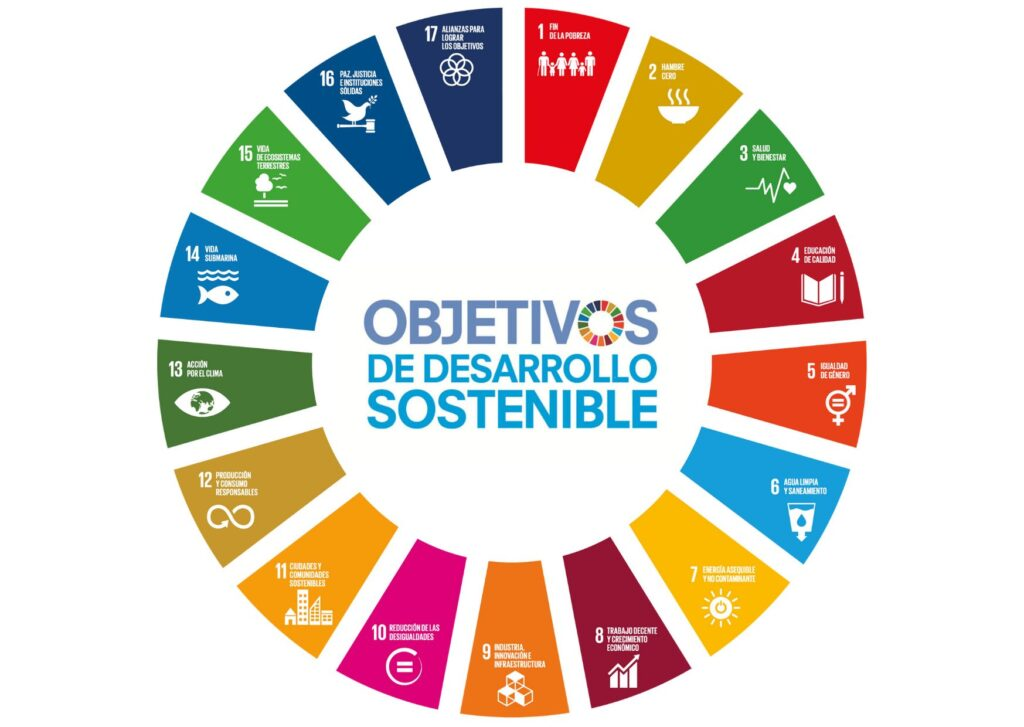
\includegraphics[width=0.7\linewidth]{img/ODS.jpg}
    \caption{Objetivos ODS del Desarrollo Sostenible}
    \label{fig:ODS}
\end{figure}

